\documentclass[tikz,border=5pt]{standalone}
\usepackage{tikz}
\usetikzlibrary{shapes.geometric,arrows.meta,positioning,shadows}

\begin{document}
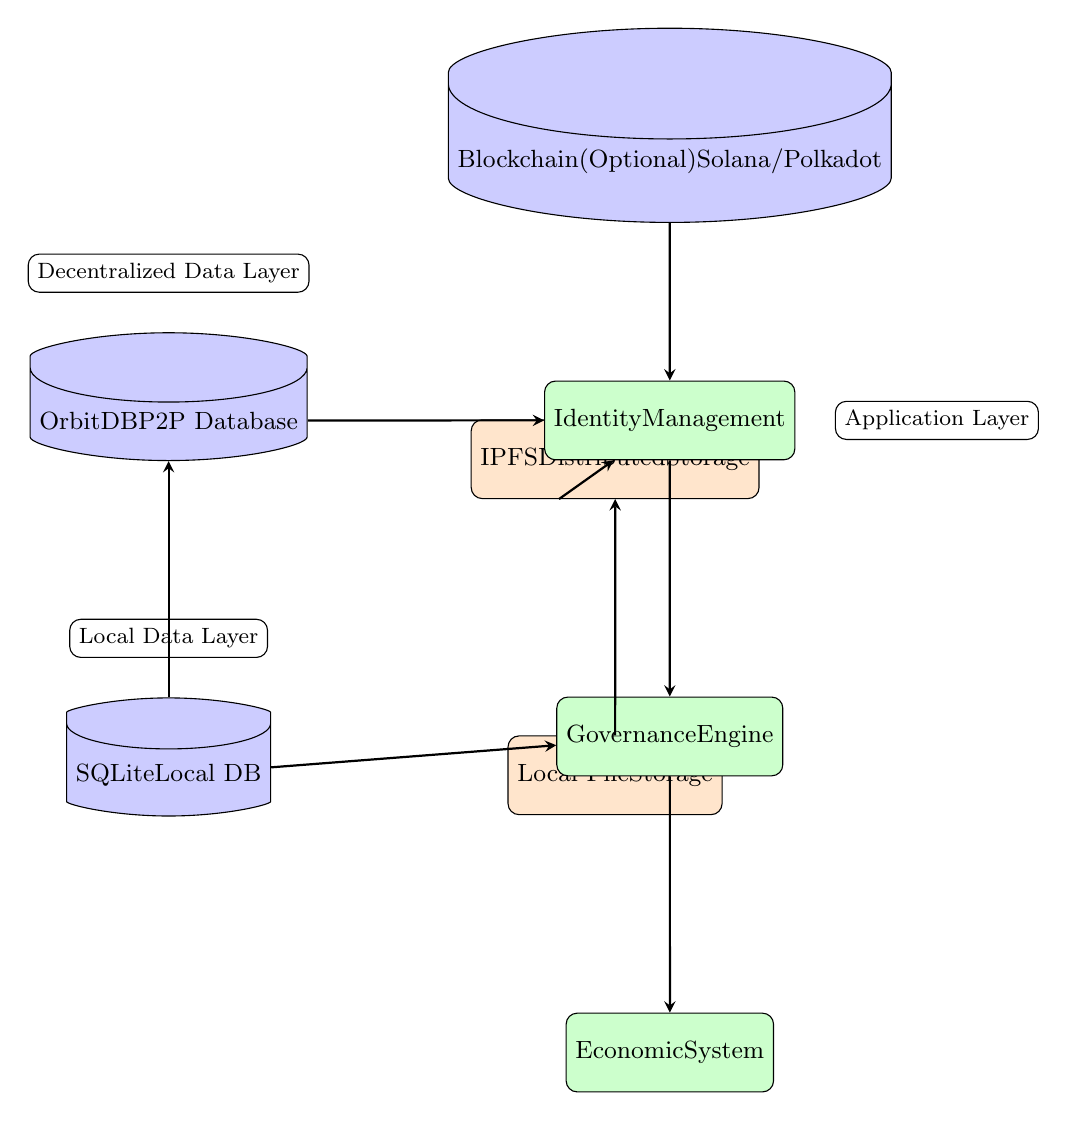
\begin{tikzpicture}[scale=1.5,
    node distance=3cm,
    every node/.style={draw,rounded corners,font=\small},
    database/.style={cylinder,shape border rotate=90,aspect=0.25,minimum height=1.5cm,minimum width=2cm,fill=blue!20},
    process/.style={rectangle,minimum width=2cm,minimum height=1cm,fill=green!20},
    storage/.style={rectangle,minimum width=2.5cm,minimum height=1cm,fill=orange!20},
    arrow/.style={->,>=stealth,thick}
]

% Local Storage Layer
\node[database] (sqlite) {SQLite\\Local DB};
\node[storage,right=of sqlite] (files) {Local File\\Storage};

% P2P Storage Layer  
\node[database,above=of sqlite] (orbitdb) {OrbitDB\\P2P Database};
\node[storage,above=of files] (ipfs) {IPFS\\Distributed\\Storage};

% Application Layer
\node[process,right=3cm of orbitdb] (identity) {Identity\\Management};
\node[process,below=of identity] (governance) {Governance\\Engine};
\node[process,below=of governance] (economy) {Economic\\System};

% Blockchain Layer (Optional)
\node[database,above=2cm of identity] (blockchain) {Blockchain\\(Optional)\\Solana/Polkadot};

% Connections
\draw[arrow] (sqlite) -- (orbitdb);
\draw[arrow] (files) -- (ipfs);
\draw[arrow] (orbitdb) -- (identity);
\draw[arrow] (ipfs) -- (identity);
\draw[arrow] (sqlite) -- (governance);
\draw[arrow] (governance) -- (economy);
\draw[arrow] (identity) -- (governance);
\draw[arrow] (blockchain) -- (identity);

% Labels
\node[above=0.5cm of orbitdb,font=\footnotesize] {Decentralized Data Layer};
\node[above=0.5cm of sqlite,font=\footnotesize] {Local Data Layer};
\node[right=0.5cm of identity,font=\footnotesize] {Application Layer};

\end{tikzpicture}
\end{document}
